\section{Use cases and requirements}

The fundamental steps in formulating use cases encompass the following:
\begin{enumerate}
    \item Assign a name to the use case.
    \item Identify the actors: generalize specific names to encompass participating actors.
    \item Focus on the flows of events, entry and exit conditions using natural language.
    \item Give due attention to exceptional cases and special requirements.
\end{enumerate}
Each use case can give rise to one or more requirements.
 
A use case represents a sequence of events within the system, involving interactions with actors. 
These use cases are initiated by an actor and conclude under specific termination conditions.
\begin{definition}[\textit{Use case model}]
    The use case model is the set of all use cases specifying the complete functionality of the system. 
\end{definition}
\begin{definition}[\textit{Requirements engineering}]
    A use case association is a relationship between use cases. 
    The primary types of use case associations include: include, extends and the generalization.
\end{definition}
\begin{figure}[H]
    \centering
    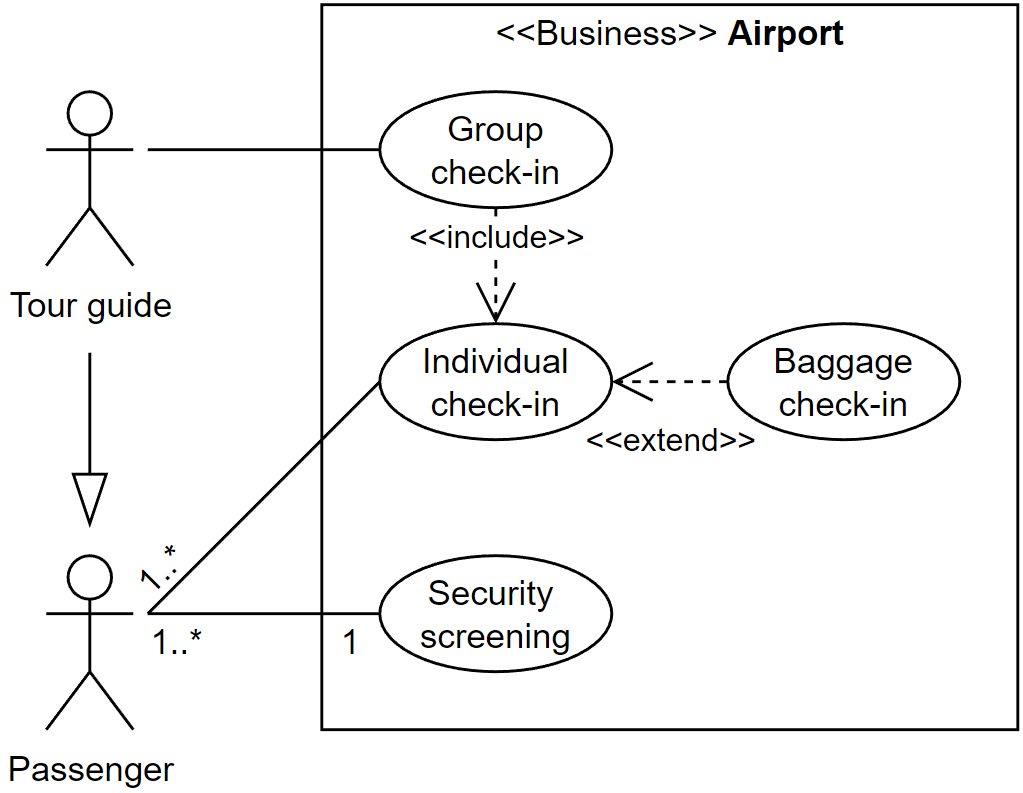
\includegraphics[width=0.5\linewidth]{images/usecase.png}
    \caption{Use case model example}
\end{figure}